\chapter{音声合成と音声\ruby{認識}{にん|しき}}
\section{この章でやること}

この章では、Rapsberry Piに言葉を話させる方法と、言葉を聞き取らせる方法を学びます。
\ruby{機械}{き|かい}に言葉を話させることを「\ruby{音声合成}{おん|せい|ごう|せい}」、機械に言葉を聞き取らせることを「\ruby{音声認識}{おん|せい|にん|しき}」と呼びます。
この教材では、音声合成にはOpenJtalk、音声認識にはJuliusというソフトウェアを使用します。
計算結果をRapsberry Piに話させたり、音声でLEDを点灯させたりしながら、Raspberry Piで音声を使った処理を実現してみましょう。

\subsection{教材を自分のフォルダに置こう}
まずは、今回利用する教材をコピーしましょう。
前回までと同じように、\nobreak/usr/local/share/ome にあるフォルダ 05 を自分のホームディレクトリにコピーしてください。

\newpage
\section{音声合成}
音声合成とは何でしょう。それは、人間の声を人工的に機械で作り出すことです。みなさんが目にするもので言えば、例えばソフトバンクが\ruby{制作}{せい|さく}するPepper(図\ref{pepper})というロボットがあります。

\begin{figure}[H]
\begin{center}
    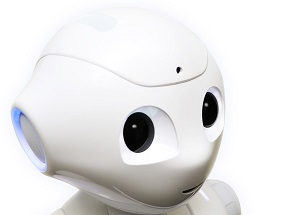
\includegraphics[width=.4\linewidth]{images/chap06/text06-img001.jpg}
    \caption{Pepper (softbank)}
    \label{pepper}
\end{center}
\end{figure}

Pepperは声を出して利用者とコミュニケーションを取ります。Pepperから声が出るのは、中に人間が入っているわけではありません。読み上げたい文章があったとき、その文章に合った音声を作り、スピーカーから\ruby{鳴}{な}らしているのです。
今回は音声を合成するために、OpenJTalkと\ruby{呼}{よ}ばれる音声合成のためのソフトウェアを使います。OpenJTalkは、読み上げたい文章と、ひらがなごとの音(\ruby{厳密}{げん|みつ}にはもう少し多種の音)を入力し、\ruby{対応}{たい|おう}する音声ファイルを出力します(図\ref{OpenJTalkの入出力})。

\begin{figure}[H]
\begin{center}
    \includesvg[width=.7\linewidth]{images/chap06/text06-img011.svg}
    \caption{OpenJTalkの入出力}
    \label{OpenJTalkの入出力}
\end{center}
\end{figure}

\begin{tcolorbox}[title=\useOmetoi]
\begin{enumerate}
        \addquiz{音声合成とはなんですか。20字以内で説明してください。}
        \addquiz{音声合成をするにはパソコンに何を\ruby{準備}{じゅん|び}する必要がありますか。3つ挙げてください。}
\end{enumerate}
\end{tcolorbox}
